\documentclass[french,12pt]{article}
\usepackage{babel}

\usepackage[utf8]{inputenc}%encodage des caractères
\usepackage[T1]{fontenc}%encodage de la police
\usepackage{graphicx}
\setlength{\parindent}{0pt} 
\usepackage{float}

\title{Rapport Complément Programmation Orientée}
\author{Amélie Phok, Antonin Montagne, Lou-Anne Gautherie, \\Naya Makdessi}
\date{8 Avril 2022}

\begin{document}

\maketitle

\begin{figure}[h]	
	\begin{center}
		
\includegraphics[scale=0.4]{img/fond.png}	
	\end{center}
\end{figure}

\begin{figure}[b]
	\begin{center}
		
\includegraphics[scale=0.7]{img/unicaen.png}	
	\end{center}
\end{figure}

\thispagestyle{empty}
\setcounter{page}{0}
\newpage

\tableofcontents
\newpage

\section{Introduction}

\subsection{Description du projet}

Nous avions pour but de coder en Java, un jeu de puzzle à glissières qui s'intitule "Taquin". Ce genre de jeu est une grille de n lignes sur m colonnes, avec n*m-1 éléments (c'est-à-dire qu'une case est vide). Le joueur a pour but faire glisser l'un des éléments contigus à la case vide vers cette dernière afin de remettre les cases dans le bon ordre.\\

\subsection{Objectifs du projet}

Nous voulions développer une interface graphique où l'on pourrait cliquer sur des boutons pour bouger la pièce vide. Nous avions d'abord pour but de dévélopper la même chose mais sur le \textbf{Terminal}; c'est-à-dire de rentrer des commandes telles que "\textit{haut}" ou encore "\textit{gauche}" pour bouger la pièce vide. 

\section{Organisation du projet}

Nous avons décidé de se répartir les tâches en suivant le concept MVC, c'est-à-dire Modèle, Vue, Contrôleur.\\

Pour commencer, Amélie a crée la classe qui définit un puzzle, nommée \textsf{ModeleTaquin}.
Antonin, Lou-Anne et Naya ont crée le reste des classes MVC qui sont:

\begin{itemize}
\item \textsf{AbstractModeleEcouteur} dans \textsf{controle}
\item \textsf{EcouteurModele} dans \textsf{controle}
\item \textsf{ModeleEcoutable} dans \textsf{controle}
\item \textsf{ModeleGUI} dans \textsf{vue}
\item \textsf{VueModel} dans \textsf{vue}
\item \textsf{Image} dans \textsf{vue}\\
\end{itemize} 

Notre modèle est donc la classe \textsf{ModeleTaquin} dans \textsf{modele} codé par Amélie. Ce modèle hérite ainsi de la classe \textsf{AbstractModeleEcouteur} qui permet d'\textit{écouter} le modèle lorqu'une pièce est bougée.
\\\\
Cette classe contient plusieurs méthodes telles que \texttt{shuffle()} qui permet de mélanger la grille un nombre aléatoire de fois ou encore \texttt{swap(int i, int j)} qui permet d'échanger une case de coordonnées (i,j) avec la case vide. 
\\\\
Enfin, la méthode \texttt{isOver()} vérifie si le puzzle est terminé.
\\\\
Pour la partie affichage de l'interface graphique, c'est Antonin qui a codé la classe \textsf{VueModel}, \textsf{Image} et \textsf{ModeleGUI}. 
\\
La classe \textsf{ModeleGUI} hérite de la classe \textsf{JFrame} est permet d'appeler les constructeur des classes \textsf{Image} et \textsf{VueModel}. Elle prend un argument une instance de \textsf{ModeleTaquin}. 
\\
La classe \textsf{Image} prend en argument le chemin de l'image que l'on veut utiliser et les dimensions de l'image final. Cette classe contient deux méthodes \texttt{redimension} qui permet de redimensionner l'image d'origine en 500*500 et \texttt{decoupe} qui permet de découper l'image en parties. 
\\
La classe {VueModel} prend en paramètre une instance de \textsf{ModeleTaquin}, le nombre de lignes et de colonnes, le nom de l'image et la JFrame. Pour afficher le jeu, il appel la méthode \texttt{affichageGrille}. Dans cette méthode, il a crée un tableau de \texttt{JButton} et une map qui contient pour chaque nombre de la grille ses coordonnées dans le modèle. Puis pour chaque nombre de la grille, il a crée un \texttt{JButton} au quel il a donné en argument le chemin de la sous-image qui correspond au numéro de la case.
Il a rendu tout les boutons sauf celui de la case vide cliquable pour pouvoir échanger la case avec la case vide. Quand le focus est sur la case vide, il a crée un évènement permettant de déplacer la case avec les flèches. A chaque déplacement, il appel la méthode \texttt{swap} du modèle. La méthode \texttt{modeleMisAJour} supprime tout les éléments de l'affichage est appel \texttt{affichageGrille}. Enfin la fonction \texttt{deleteImg} permet de supprimer toutes les sous-images crée une fois la partie gagné.
\\\\
Pour la partie Terminal, c'est Lou-Anne qui a commencé à coder la classe \textsf{Terminal}, utilisant la classe \texttt{Scanner} de Java.\\
Elle a implémenté ce qu'Amélie avait fait dans \textsf{ModeleTaquin} pour importer un taquin aléatoire définit sur 3 par 3.\\
Elle a créé un \texttt{Scanner} qui récupère la commande rentrée par l'utilisateur, c'est-à-dire "\textit{haut}", "\textit{bas}", \textit{droite}", ou "\textit{gauche}".\\
Si la commande rentrée n'existe pas, le terminal redemande de saisir une commande correcte. \\
Elle a ensuite fait des conditions de sorte d'associer la commande rentrée, avec l'échange correspondant (avec la méthode \texttt{swap()} de la classe \textsf{ModeleTaquin}). Sauf que les coordonnées codées par Lou-Anne n'étaient pas les bonnes, Naya a donc prit le relais et a mis les coordonnées correspondantes aux échanges. Elle a aussi fait en sorte que si il y a un mur là où l'utilisateur voulait mettre la pièce vide, le terminal redemande au joueur de rentrer une commande correcte.\\

\section{Architecture du projet}

Ce premier diagramme montre comment nous avons organisé l'architecture de notre projet en différents paquets.\\
Comme on peut le voir, le paquet \textsf{controle} contient les éléments de controle abstrait mais aussi les classes \textsf{Terminal} et \textsf{Fenetre} qui permettent de lancer le jeu dans le terminal et dans une interface graphique respectivement.

\begin{figure}[H]
    \begin{center}
    	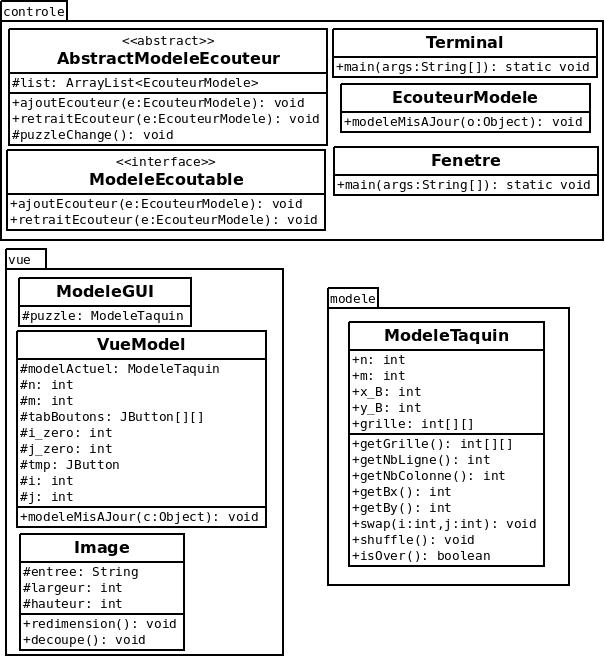
\includegraphics[scale=0.4]{img/packages.jpg}
    \end{center}
    \caption{Diagrammes des paquets utilisés pour le projet}
\end{figure}

Ce deuxième diagramme permet d'illustrer le concept MVC et comment les trois parties dépendent les unes des autres. 

\begin{figure}[H]
    \begin{center}
    	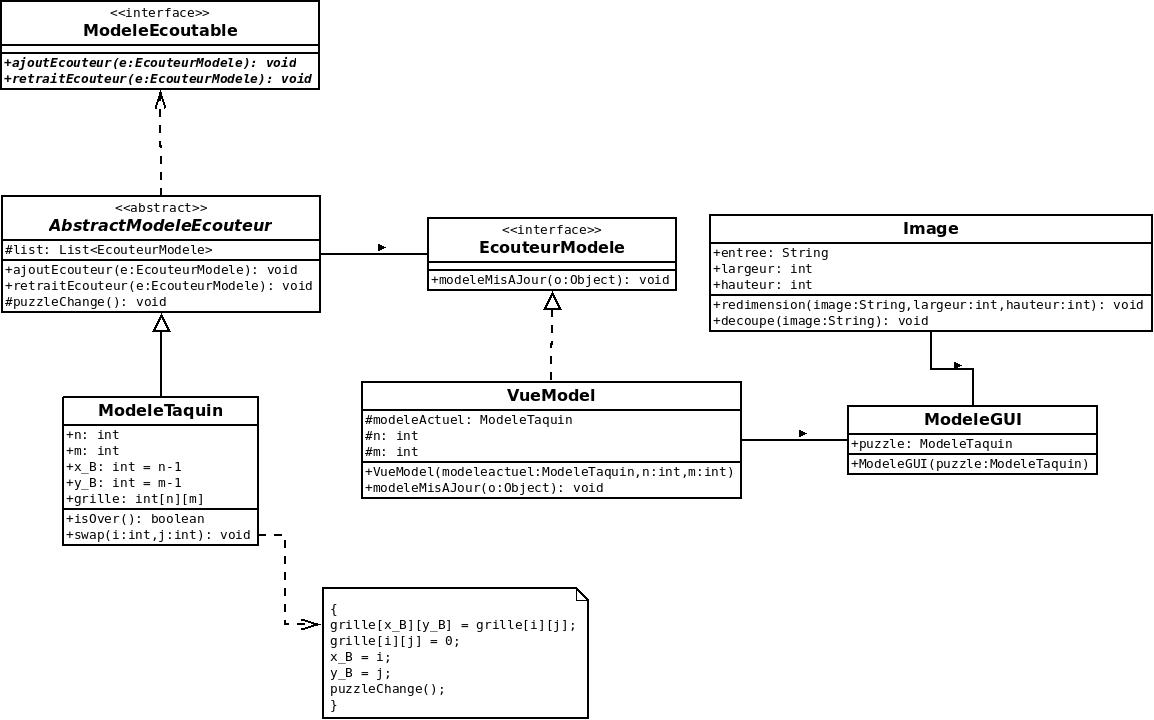
\includegraphics[scale=0.2]{img/classes.jpg}
    \end{center}
    \caption{Diagramme des classes avec leurs dépendances}
\end{figure}

\section{Documentations}

La documentation a été générée automatiquement avec les commentaires Javadoc formatés avec /** et */.\\
Dans le dossier \textsf{doc}, c'est la page index.html qui permet d'accéder à l'ensemble de la documentation ainsi générée.

\section{Expérimentations}

Le jeu peut être lancé à partir de deux fichiers .jar qui sont a exécutés directement dans le dossier \textsf{dist}.
\\\\
\texttt{TaquinTerminal.jar} lance le jeu dans le terminal et \texttt{TaquinInterface.jar} lance le jeu dans une fenêtre graphique.
\\\\
Lorsque vous lancez le jeu, avec \texttt{runTerminal}, le Terminal affiche la grille mélangée et vous demande de saisir une commande:

\begin{center}
	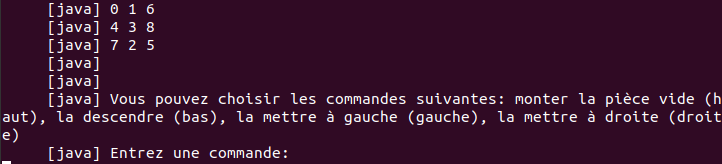
\includegraphics[scale=0.3]{img/terminal.png}
\end{center}

Lorsque vous lancez le jeu, avec \texttt{runInterface}, une fenêtre s'ouvre, vous demandant de saisir le nom de l'image que vous voulez jouer (se trouvant dans le répertoire image). L'image apparait découpée, il faut cliquer sur une case pour placer la case vide à l'endroit du clique. On peut aussi cliquer sur la case vide et la bouger avec les flèches.

\begin{center}
	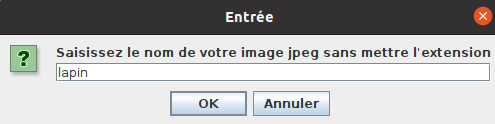
\includegraphics[scale=0.3]{img/titreImg.png}\\
	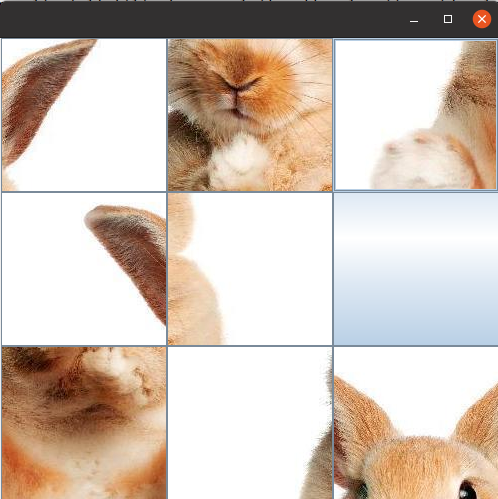
\includegraphics[scale=0.3]{img/imgDecoupee.png}
\end{center}

\section{Conclusion}

Nous avons ainsi complété la majorité des objectifs de notre projet.
Notre puzzle est en effet construit selon le concept MVC avec une partie Modèle, Vue et Contrôleur.

Il est possible de jouer avec des commandes textes dans le terminal ou de jouer dans une interface graphique avec une image à reconstituer.

\end{document}